\pagestyle{fancy}
\setlength{\headheight}{16pt}
\fancyhead{} % clear all header fields
\fancyhead[L]{\textbf{CEE 576 Midterm}}
\fancyhead[C]{Songyuan Cui}
\fancyhead[R]{\textbf{Fall 2024}}
\fancyfoot{} % clear all footer fields
\fancyfoot[C]{\thepage}

\newcommand{\ca}[1]{\textcolor{Maroon}{#1}}
\newcommand{\cb}[1]{\textcolor{RoyalBlue}{#1}}
\newcommand{\cc}[1]{\textcolor{PineGreen}{#1}}
\newcommand{\cd}[1]{\textcolor{Plum}{#1}}

\newcommand{\Fint}{\ensuremath{\bv{F}^{\textrm{int}}}}
\newcommand{\Fext}{\ensuremath{\bv{F}^{\textrm{ext}}}}

\section*{Q1}
The result (\cref{fig:midterm_p1}) matches the provided figures. 
Displacement at node 3 (upper left corner) is $u = \qty{-2e-6}{}, v = \qty{-4e-6}{}$. 
\begin{figure}[!ht]
\centering
\begin{subfigure}{0.45\textwidth}
    \centering
    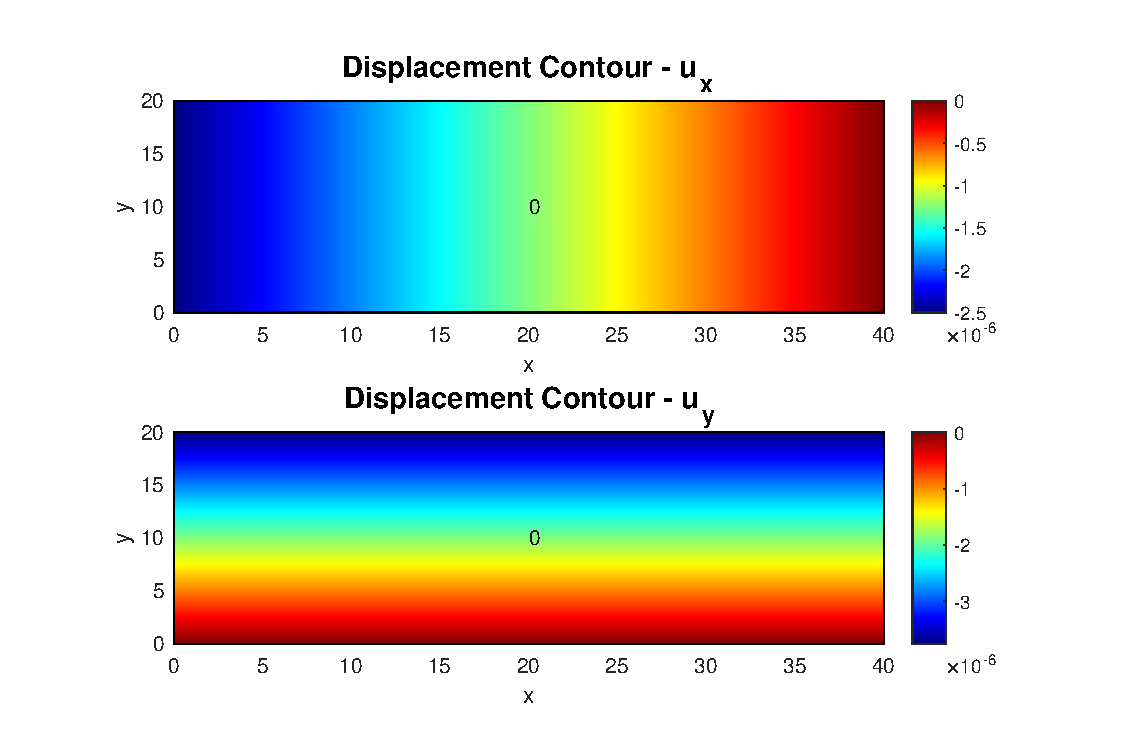
\includegraphics[width=\textwidth]{midterm/midterm_p1_contour.pdf}
    \caption{Displacement contours}
\end{subfigure}
\begin{subfigure}{0.45\textwidth}
    \centering
    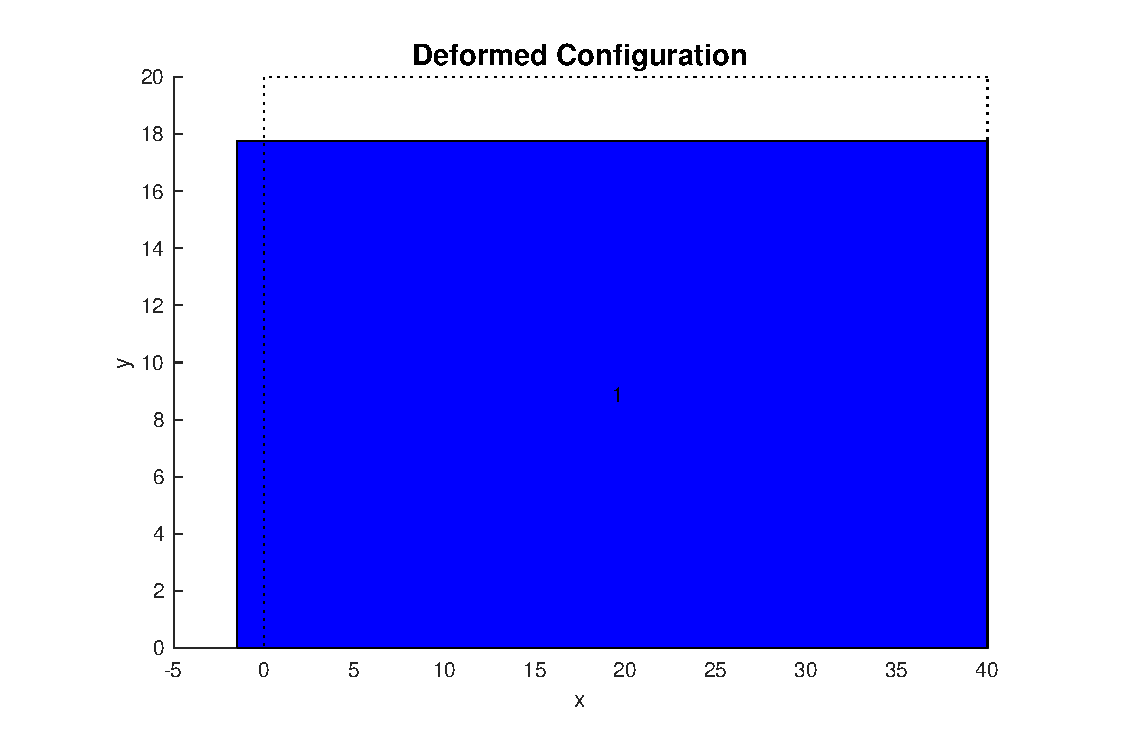
\includegraphics[width=\textwidth]{midterm/midterm_p1_deform.pdf}
    \caption{Deformed configuration (upscaled)}
\end{subfigure}
\caption{Linear elasticity validation using two triangular elements}
\label{fig:midterm_p1}
\end{figure}

\section*{Q2}
\begin{enumerate}[(a)]
\item {
    The strain energy density function is given as 
    \begin{equation}
        W(\bt{\varepsilon}) = \frac{1}{2}a \varepsilon_{mm} \varepsilon_{nn} + \frac{1}{2}b \varepsilon_{mn} \varepsilon_{mn} + \frac{1}{3}c \varepsilon_{mn}\varepsilon_{np}\varepsilon_{mp}
    \end{equation}
    where $\bt{\varepsilon}$ is the symmetric infinitesimal strain tensor.
    In general, for symmetric tensors such as $\epsilon_{ij}$, we have its partial derivative 
    \begin{equation}
        \frac{\partial \varepsilon_{ij}}{\partial \varepsilon_{kl}} = \frac{1}{2}\left(\delta_{ik}\delta_{jl} + \delta_{il} \delta_{jk} \right)
    \end{equation}
    It immediately follows that 
    \begin{equation}
        \frac{\partial \varepsilon_{mm}}{\partial \varepsilon_{ij}} = \delta_{ij}
    \end{equation}
    Hence, the Cauchy stress tensor is 
    \begin{equation}
    \begin{aligned}
        \sigma_{ij} &= \frac{\partial W}{\partial \varepsilon_{ij}} \\
        &= a \varepsilon_{mm} \delta_{ij} + b\varepsilon_{mn} \cdot \frac{1}{2}(\delta_{mi}\delta_{nj} + \delta_{mj}\delta_{ni}) + c\varepsilon_{np} \varepsilon_{mp} \cdot \frac{1}{2}(\delta_{mi}\delta_{nj} + \delta_{mj}\delta_{ni}) \\
        &= a \varepsilon_{mm} \delta_{ij} + b\varepsilon_{ij} + c\varepsilon_{ip} \varepsilon_{jp} \\
        &= {\left[a \textrm{tr}(\bt{\varepsilon})\bt{1} + b\bt{\varepsilon} + c \bt{\varepsilon}\bt{\varepsilon} \right]}_{ij}  \\
    \end{aligned}
    \end{equation}
    which is a more compact form of the provided expression leveraging the symmetry of $\epsilon_{ij}$.
    The material moduli tensor is then 
    \begin{equation}
    \begin{aligned}
        c_{ijkl} &= \frac{\partial^2 W}{\partial \varepsilon_{ij} \partial \varepsilon_{kl}} \\
        &= a\delta_{ij}\delta_{kl} + \frac{1}{2}b\left(\delta_{ik}\delta_{jl} + \delta_{il} \delta_{jk} \right) + c \varepsilon_{jp}
        \cdot \frac{1}{2}\left(\delta_{ik}\delta_{pl} + \delta_{il} \delta_{pk} \right) 
        + c \varepsilon_{ip}
        \cdot \frac{1}{2}\left(\delta_{jk}\delta_{pl} + \delta_{jl} \delta_{pk} \right) \\
        &= a\delta_{ij}\delta_{kl} + \frac{1}{2}b\left(\delta_{ik}\delta_{jl} + \delta_{il} \delta_{jk} \right) + \frac{1}{2} c \left(
            \ca{\delta_{ik}\varepsilon_{jl}} + 
            \cb{\delta_{il}\varepsilon_{jk}} + 
            \cc{\delta_{jk}\varepsilon_{il}} + 
            \cd{\delta_{jl}\varepsilon_{ik}} 
        \right)
    \end{aligned}
    \end{equation}
    which can be matched to the given expression by expanding $\varepsilon_{ij}= (\varepsilon_{ij} + \varepsilon_{ji})/2$.
} 
\item {
Using the symmetry of $\delta_{ij}$ and $\varepsilon_{ij}$:
\begin{subequations}
\begin{equation}
    c_{klij} = a\delta_{kl}\delta_{ij} + \frac{1}{2}b\left(\delta_{ki}\delta_{lj} + \delta_{kj} \delta_{il} \right) + \frac{1}{2} c \left(
        \ca{\delta_{ki}\varepsilon_{lj}} + 
        \cc{\delta_{kj}\varepsilon_{li}} + 
        \cb{\delta_{li}\varepsilon_{kj}} + 
        \cd{\delta_{lj}\varepsilon_{ki}}
    \right) = c_{ijkl}
\end{equation}
\begin{equation}
    c_{jikl} = a\delta_{ji}\delta_{kl} + \frac{1}{2}b\left(\delta_{jk}\delta_{il} + \delta_{jl} \delta_{ik} \right) + \frac{1}{2} c \left(
        \cc{\delta_{jk}\varepsilon_{il}} + 
        \cd{\delta_{jl}\varepsilon_{ik}} + 
        \ca{\delta_{ik}\varepsilon_{jl}} + 
        \cb{\delta_{il}\varepsilon_{jk}} 
    \right) = c_{ijkl}
\end{equation}
\begin{equation}
    c_{ijlk} = a\delta_{ij}\delta_{lk} + \frac{1}{2}b\left(\delta_{il}\delta_{jk} + \delta_{ik} \delta_{jl} \right) + \frac{1}{2} c \left(
        \cb{\delta_{il}\varepsilon_{jk}} + 
        \ca{\delta_{ik}\varepsilon_{jl}} + 
        \cd{\delta_{jl}\varepsilon_{ik}} + 
        \cc{\delta_{jk}\varepsilon_{il}} 
    \right) = c_{ijkl}
\end{equation}
\end{subequations}
which shows that $c_{ijkl}$ exhibits both major and minor symmetry. 
}
\item {
For 2D plane strain, $\varepsilon_{33}=\varepsilon_{13}=\varepsilon_{31}=0$.
Hence, 
\begin{equation}\label{eqn:midterm_D}
\begin{aligned}
    \begin{bmatrix}
        \sigma_{11}' \\ \sigma_{22}' \\ \sigma_{12}'
    \end{bmatrix} &= \begin{bmatrix}
        c_{1111} & c_{1122} & c_{1112} \\
        c_{2211} & c_{2222} & c_{2212} \\
        c_{1211} & c_{1222} & c_{1212}
    \end{bmatrix} \begin{bmatrix}
        \varepsilon_{11} \\ \varepsilon_{22} \\ 2\varepsilon_{12}
    \end{bmatrix} \\ 
    &= \underbrace{\begin{bmatrix}
        a + b + 2c\varepsilon_{11}  & a & c \varepsilon_{12} \\
         & a + b + 2c\varepsilon_{22} & c \varepsilon_{12}  \\
        \textrm{Sym.} &  & \frac{1}{2}b + \frac{1}{2}c(\varepsilon_{11} + \varepsilon_{22})
    \end{bmatrix}}_{\bt{D}} \begin{bmatrix}
        \varepsilon_{11} \\ \varepsilon_{22} \\ 2\varepsilon_{12}
    \end{bmatrix}
\end{aligned}
\end{equation}
where $\sigma_{ij}'$ are pseudo-stress that are not physically meaningful.
In addition, $\sigma_{33}' = a(\varepsilon_{11} + \varepsilon_{22})$.
This differs from linear elasticity only by the nonlinear term $c \bt{\varepsilon} \bt{\varepsilon}$, and $a$, $b$ correspond to Lam\'{e}'s first ($\lambda$) and second ($\mu$) parameters, respectively. 
}
\end{enumerate}

\section*{Q3}
\begin{enumerate}[(a)]
\item { % 3(a)
Given the domain $\Omega$, Dirichlet and Neumann boundaries $\Gamma_{g,i}, \Gamma_{h,i}$ and corresponding values $g_i, h_i$, and the constitutive coefficients $a, b, c$, the \emph{strong form} for small nonlinear strain is written as 
\begin{subequations}
\begin{align}
    \sigma_{ij,j} + f_i &= 0, ~~~~~ \bv{x} \in \Omega \\
    u_i &= g_i, ~~~~ \bv{x} \in \Gamma_{g,i} \\
    \sigma_{ij} n_j &= h_i, ~~~~ \bv{x} \in \Gamma_{h,i} \\
    \sigma_{ij} &= \sigma_{ij}(\bt{\varepsilon}; a, b, c)
\end{align}
\end{subequations}
} 
\item { % 3(b)
Define the trial and test space:
\begin{equation}
\begin{aligned}
    \mathcal{S}_i &= \left \{ u_i \in \mathcal{H}^1 ~|~ u_i = g_i ~\textrm{on}~ \Gamma_{g,i} \right \}, \\
    \mathcal{V}_i &= \left \{ w_i \in \mathcal{H}^1 ~|~ w_i = 0 ~\textrm{on}~ \Gamma_{g,i} \right \},
\end{aligned}
\end{equation}
where $\mathcal{H}^1$ represents the order-1 Sobolev space (a Hilbert space of functions whose gradients and themselves are square-integrable).
Specifically, the trial space $\mathcal{S}_i$ is \emph{the space within which we wish to find the final solution}, and hence it must satisfy the boundary conditions. Note that this space is not linear (addition of functions is no longer in the same space), and there are separate spaces for each component of $\bv{u}$. 
The test space $\mathcal{V}_i$ is \emph{the space of admissiable virtual displacements (variations)} to a given configuration. 
This requires the variations to be zero component-wise at the corresponding Dirichlet boundaries. 

The weak form is formulated as follows: find $u_i \in \mathcal{S}_i$ such that $\forall w_i \in \mathcal{V}_i$, 
\begin{equation}
    \int_\Omega w_i \sigma_{ij,j} dV + \int_\Omega w_i f_i dV = 0
\end{equation}
Integration by parts and rearranging yield 
\begin{equation}
    \int_\Omega w_{i,j} \sigma_{ij} dV = \int_\Omega w_i f_i dV + \sum_{i=1}^2 \int_{\Gamma_{h,i}} w_i h_i dA
\end{equation}
or in abstract form:
\begin{equation}
    \Fint(\bv{u}) = a(\bv{w}, \bv{u}) = (\bv{w}, \bv{f}) + {(\bv{w}, \bv{h})}_{\Gamma_{h}} = \Fext
\end{equation}
}
\item { % 3(c)
The \matlab~source code can be found at \url{https://github.com/sy-cui/CSE552-FA2024/tree/c04ab3122ea2a02fc06ec6a7ca4273ec5cab4077/midterm}.
In the same directory is attached a \texttt{README.md} file that includes summary of scripts and a brief instruction on how to reproduce the figures in Problem 4. 
}
\item { % 3(d)
The flow chart is shown in \cref{fig:midterm_flow_chart}.
The general procedure, excluding the nonlinear solution part, is form-identical to the linear elasticity program. 
Portions that are modified are marked in \textcolor{Maroon}{dark red}.
For details, see the next section (e).
}
\item { % 3(e)
In this section, we detail the modifications made to the code shown in \cref{fig:midterm_flow_chart}:
\begin{itemize}
    \item {
        We are using \emph{modified Newton-Raphson} method to solve for the nonlinear solution at multiple load steps. This outer loop is implemented in a new script \href{https://github.com/sy-cui/CSE552-FA2024/blob/c04ab3122ea2a02fc06ec6a7ca4273ec5cab4077/midterm/load_driver.m}{\texttt{load\_driver.m}} which executes the major steps (read inputs, run load steps, post process, etc.).
    }
    \item {
        Due to the now different constitutive relation, the \emph{tangent matrix} $K$ must now be modified. 
        The element-level $\bt{K}$ matrix is 
        \begin{equation}
            \bt{K}_e = \sum_{i=1}^{Nq} w_i (\bt{B}^T \bt{D} \bt{B})\Big|_{z_i}J
        \end{equation}
        where $z_i, w_i$ correspond to the $N_q$ quadrature nodes and weights, $J$ is the Jacobian, $\bt{B}$ is the gradient matrix for plane stress/strain, and $\bt{D}$ is the elastic moduli tensor given in \cref{eqn:midterm_D}.
        Evidently, this now \emph{requires the displacement field as an input} to compute the strain fields ($\bt{\epsilon} = \bt{B}\bar{\bv{u}}$). 
        The implementation can be found in \href{https://github.com/sy-cui/CSE552-FA2024/blob/c04ab3122ea2a02fc06ec6a7ca4273ec5cab4077/midterm/L_Elem2_2d.m}{\texttt{L\_Elem2\_2d.m}} where the computation of $\bt{D}$ is moved inside the integration loop.  
        
        The assembly remains identical to linear elasticity. 
        The global tangent matrix is only updated every load step, as per modified Newton method. 
        This can be easily converted to Newton-Raphson by calling \href{https://github.com/sy-cui/CSE552-FA2024/blob/c04ab3122ea2a02fc06ec6a7ca4273ec5cab4077/midterm/SolveFE.m}{\texttt{FormFE.m}} inside the solution loop in \href{https://github.com/sy-cui/CSE552-FA2024/blob/c04ab3122ea2a02fc06ec6a7ca4273ec5cab4077/midterm/SolveFE.m}{\texttt{SolveFE.m}} with properly parsed displacement input (the code in included but commented out). 
    }
    \item {
        The \href{https://github.com/sy-cui/CSE552-FA2024/blob/c04ab3122ea2a02fc06ec6a7ca4273ec5cab4077/midterm/SolveFE.m}{\texttt{SolveFE.m}} routine now uses the modified Newton-Raphson iteration. 
        An overview of the procedures is readily listed in the flow chart \cref{fig:midterm_flow_chart}. 
        Note that the linear problem can also be solved by this routine in only one step.
    }
    \item {
        The residual, defined as $\bv{r} = \Fext - \Fint(\bv{u})$, requires an additional function to compute $\Fint$.
        This is implemented in a new script \href{https://github.com/sy-cui/CSE552-FA2024/blob/c04ab3122ea2a02fc06ec6a7ca4273ec5cab4077/midterm/FintStressStrain.m#L95}{\texttt{FintStressStrain.m}}, which in additional to compute the $\Fint$ vector also outputs the stress and strain at every quadrature point. 
        This script (1) loops through every element and extract nodal position and displacements, (2) loop through quadrature nodes, (3) compute strain and then stress at the element level, (4) sum to $\Fint$ via quadrature, and (5) assemble to a global vector with Dirichlet boundaries accounted for. 
        The stresses are computed from strain as 
        \begin{equation}
        \begin{aligned}
            \sigma_{11} &= a(\varepsilon_{11}+\varepsilon_{22}) + b\varepsilon_{11} + c(\varepsilon_{11}^2 + \varepsilon_{12}^2) \\
            \sigma_{22} &= a(\varepsilon_{11}+\varepsilon_{22}) + b\varepsilon_{22} + c(\varepsilon_{12}^2 + \varepsilon_{22}^2) \\
            \sigma_{12} &= b\varepsilon_{12} + c\varepsilon_{12}(\varepsilon_{11} + \varepsilon_{22})
        \end{aligned}
        \end{equation}
        and $\Fint$ is computed as 
        \begin{equation}
            \Fint(\bv{u}) = \sum_{i=1}^{N_q} w_i J \bt{B}^T {[\sigma_{11}, \sigma_{22}, \sigma_{12}]}^T
        \end{equation}
    }
\end{itemize}
}
\end{enumerate}

\section*{Q4}
In Problem 4, we examine two simple cases representing pure stretch and pure shear. 
For both cases, a single quadrilateral element is used for a $1 \times 1$ square mesh. 
The relative tolerance is set to $\epsilon = \qty{e-9}{}$.
The material property parameters are $a = 40$, $b = 80$, and $c = 160$. 

\Cref{fig:midterm_p4_stretch} shows the stress-strain curve in the vertical direction ($\sigma_{22}$ vs $\varepsilon_{22}$) up to $5\%$ strain over 20 equally-spaced load steps for Problem 4(a). 
In this case, there is no shear ($\varepsilon_{12} = 0$) and thus a relatively simple nonlinear equation can be formulated and solved using the \matlab~\texttt{fsolve} function. 
As shown in \cref{fig:midterm_p4_stretch}, the FEM results agree well quantitatively against \matlab-computed solution. 

The stress-strain curves for Problem 4(b) are shown in \cref{fig:midterm_p4_shear}. 
In this case, there are non-trivial stress strain components in both shear and axial directions. 
The three stress components are plotted against shear strain $\varepsilon_{12}$. 
As is shown in the figure, the axial stresses remain close to zero while the shear stress increase almost linearly
This is expected as nonlinearity in the shear component arises from $\varepsilon_{11}$ and $\varepsilon_{22}$ which are relatively small in the present range. 
\begin{figure}[!ht]
    \centering
    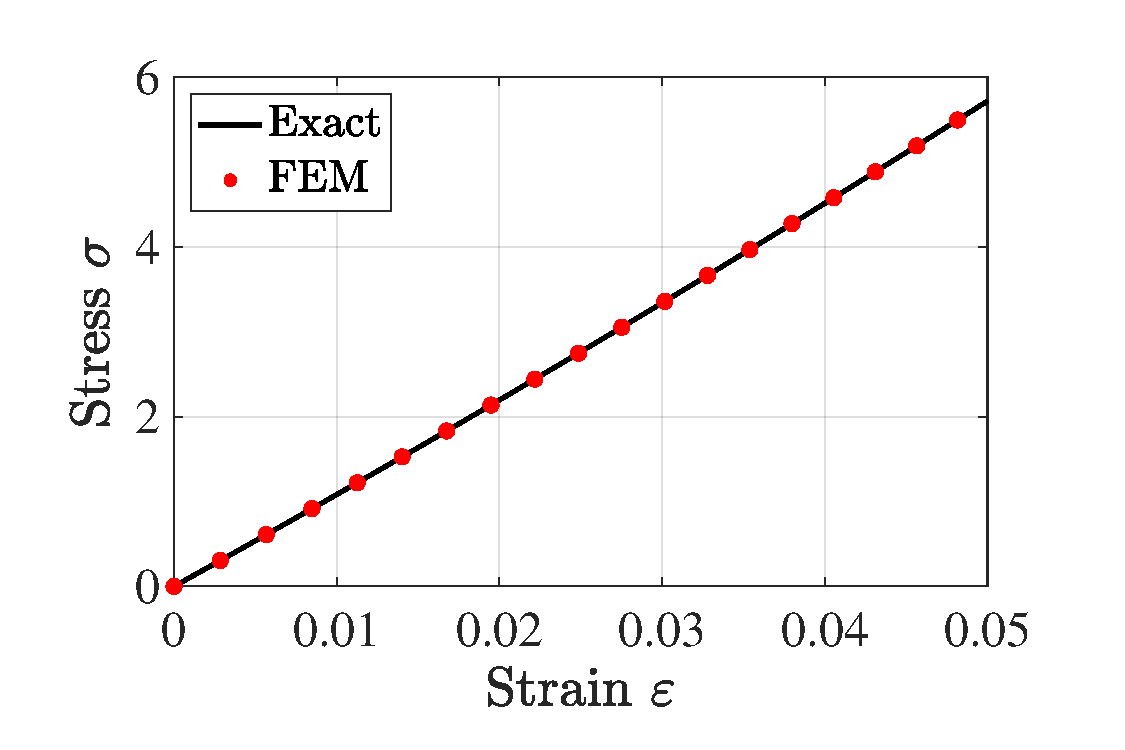
\includegraphics[width=0.6\textwidth]{midterm/midterm_p4_stretch.pdf}
    \caption{Problem 4(a) stress-strain curve in the vertical direction at the first integration point. 
    The black line is the exact solution while red dots are the converged solutions of 20 FEM load steps. }
    \label{fig:midterm_p4_stretch}
\end{figure}

\begin{figure}[!ht]
    \centering
    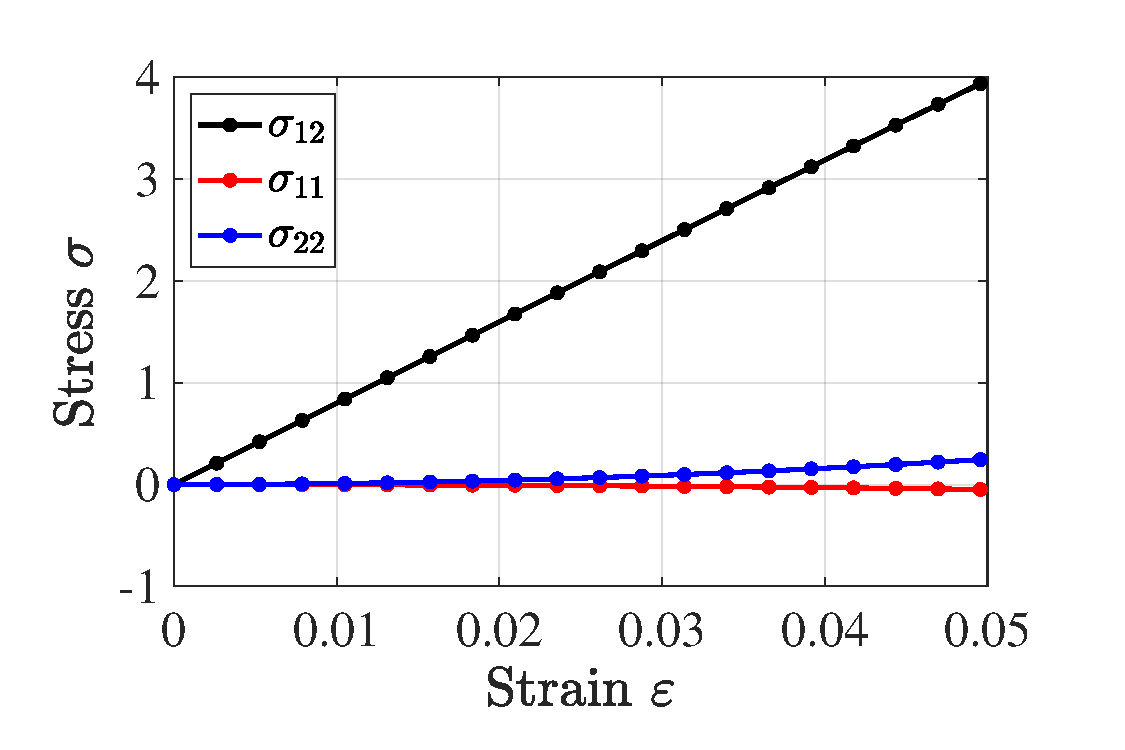
\includegraphics[width=0.6\textwidth]{midterm/midterm_p4_shear.pdf}
    \caption{Problem 4(b) stress-strain curve with respect to shear strain $\varepsilon_{12}$ at the first integration point. Dots are converged solutions of 20 FEM load steps.}
    \label{fig:midterm_p4_shear}
\end{figure}

\newpage
\begin{figure}[!ht]
    \centering
    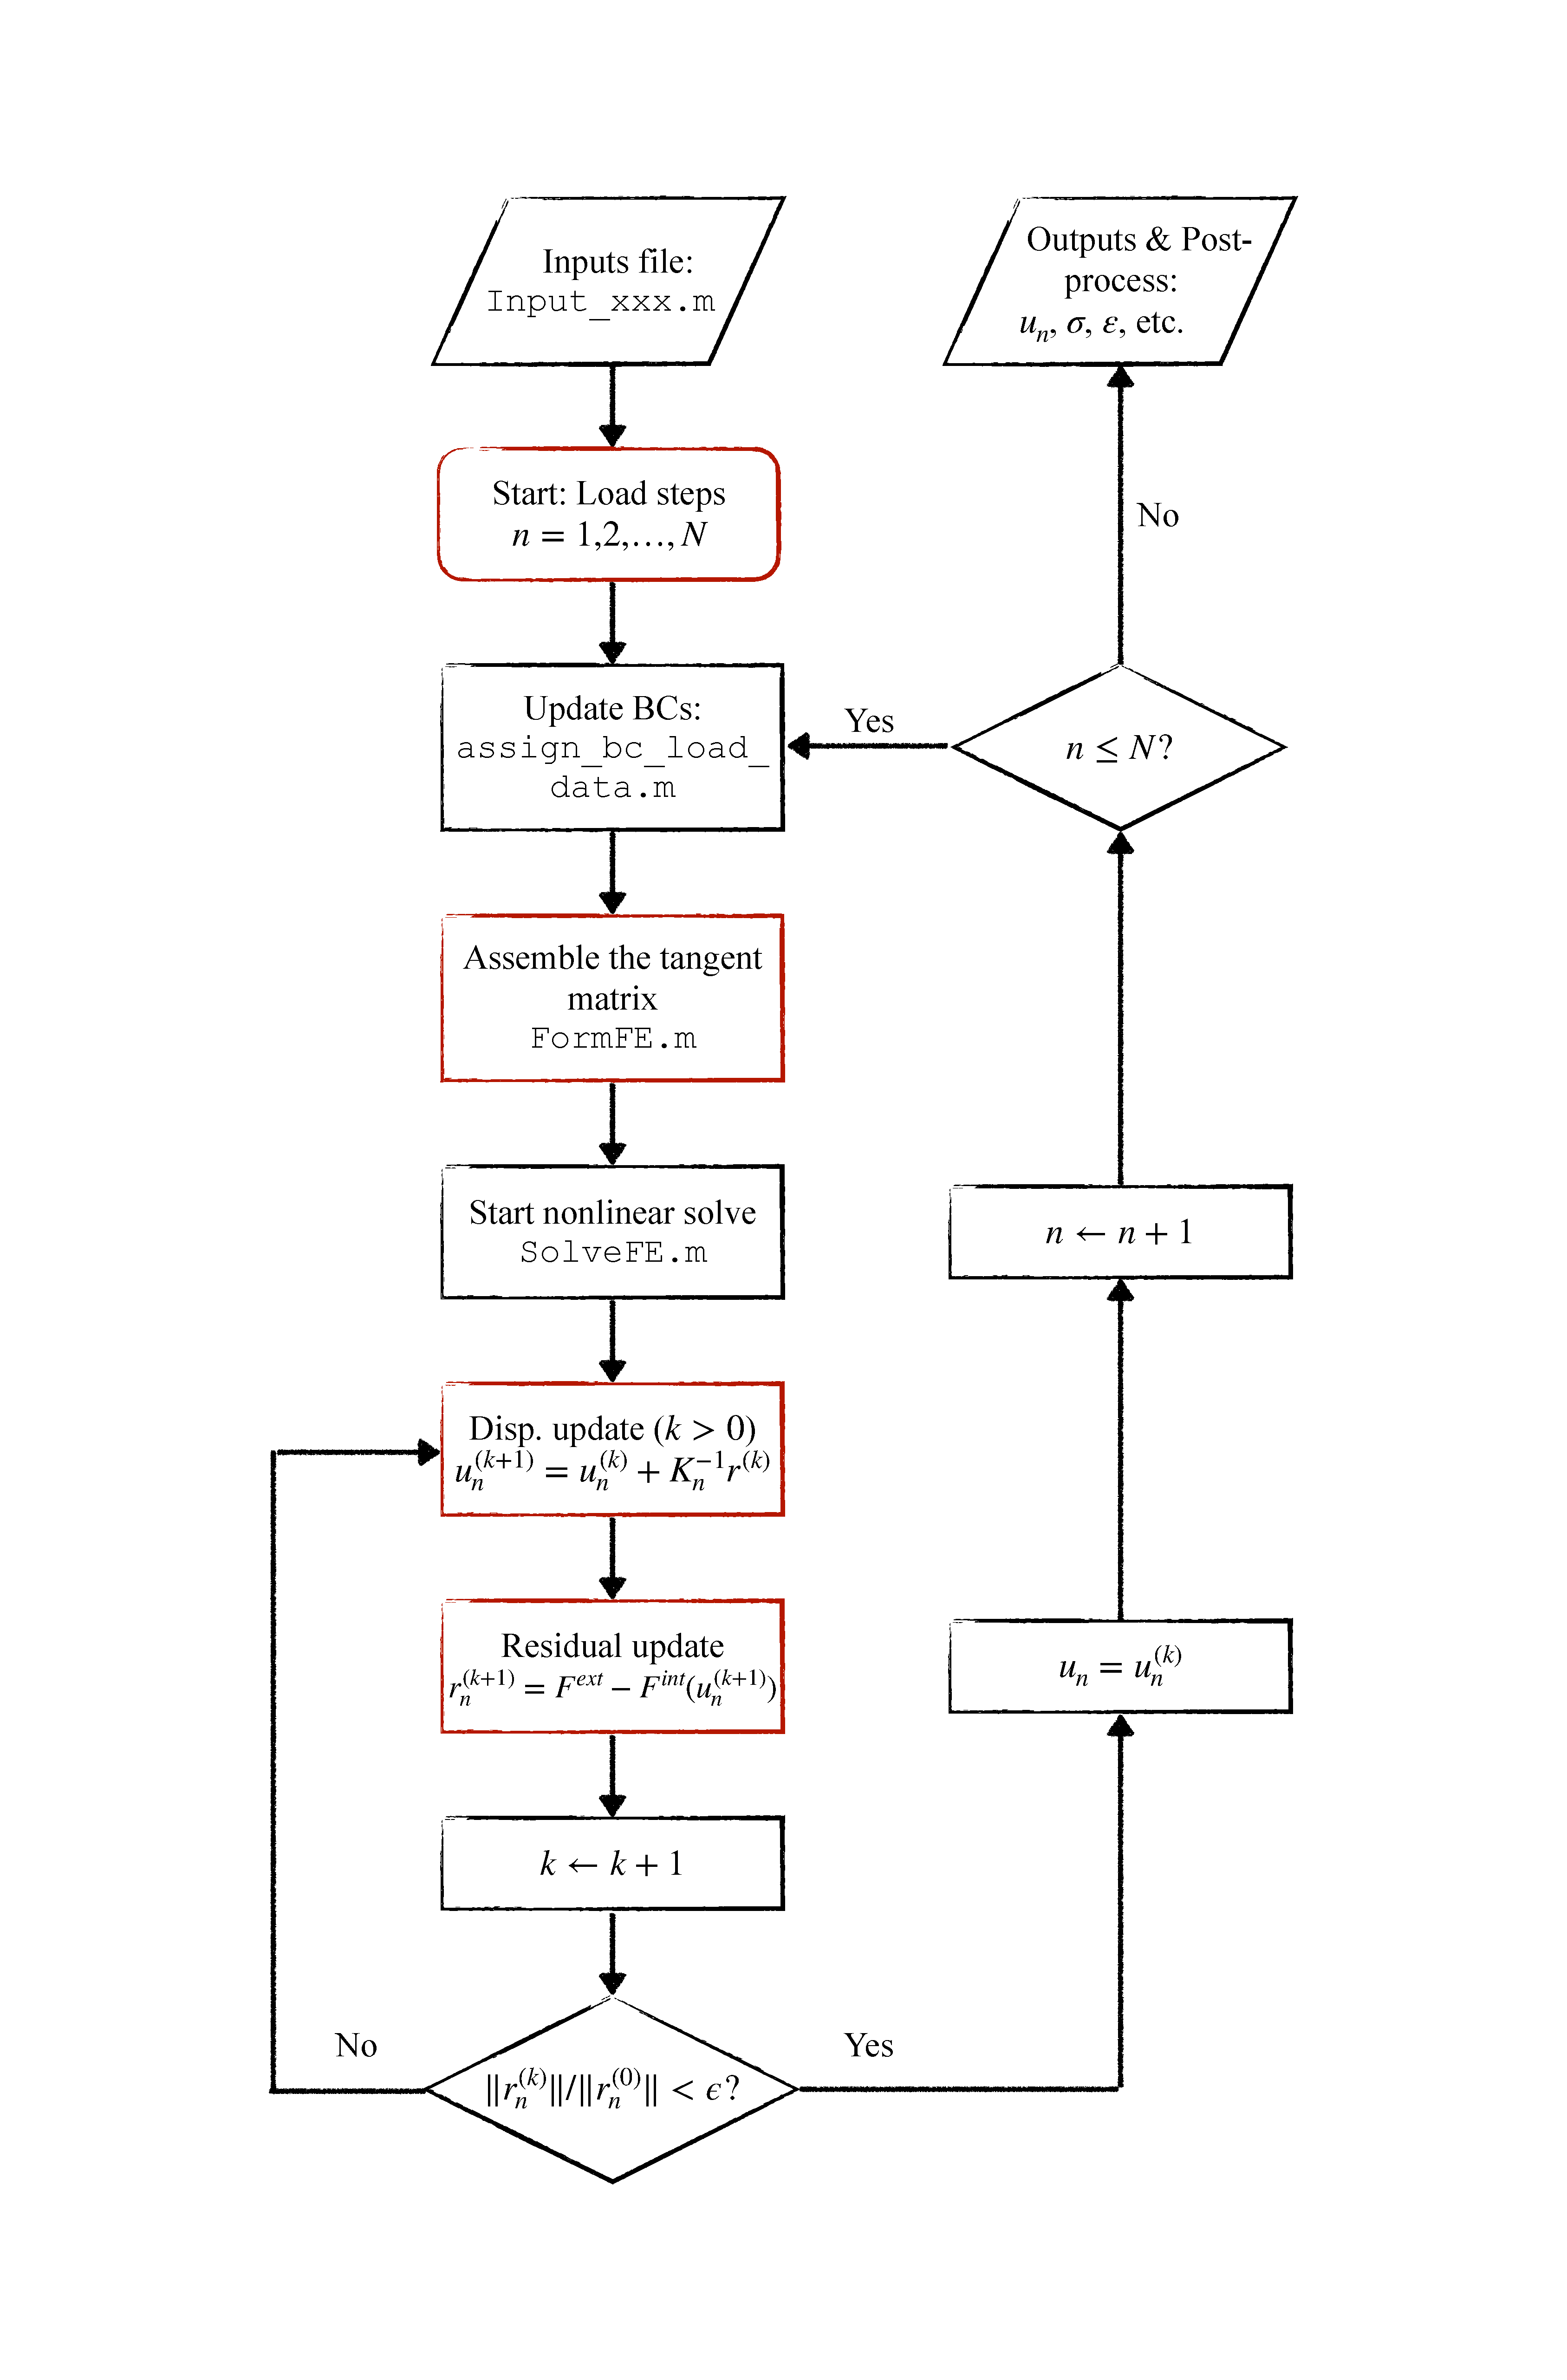
\includegraphics[width=0.9\linewidth]{midterm/flow_chart.pdf}
    \caption{Modified Newton method for material-nonlinear-only elastostatics.}
    \label{fig:midterm_flow_chart}
\end{figure}
